\documentclass{article}
\usepackage{fancyhdr}
\usepackage{extramarks}
\usepackage{amsmath}
\usepackage{amsthm}
\usepackage{amsfonts}
\usepackage{tikz}
\usepackage[plain]{algorithm}
\usepackage{algpseudocode}
\usepackage{listings} 
\usepackage{amssymb}
\usetikzlibrary{automata,positioning}

\usepackage{color}

\definecolor{dkgreen}{rgb}{0,0.6,0}
\definecolor{gray}{rgb}{0.5,0.5,0.5}
\definecolor{mauve}{rgb}{0.58,0,0.82}

\lstset{frame=tb,
  language=Python,
  aboveskip=3mm,
  belowskip=3mm,
  showstringspaces=false,
  columns=flexible,
  basicstyle={\small\ttfamily},
  numbers=none,
  numberstyle=\tiny\color{gray},
  keywordstyle=\color{blue},
  commentstyle=\color{dkgreen},
  stringstyle=\color{mauve},
  breaklines=true,
  breakatwhitespace=true,
  tabsize=3
}
%
% Basic Document Settings
%

\topmargin=-0.45in
\evensidemargin=0in
\oddsidemargin=0in
\textwidth=6.5in
\textheight=9.0in
\headsep=0.25in

\linespread{1.1}

\pagestyle{fancy}
\lhead{\hmwkAuthorName}
\chead{\hmwkClass\: \hmwkTitle}
\rhead{\firstxmark}
\lfoot{\lastxmark}
\cfoot{\thepage}

\renewcommand\headrulewidth{0.4pt}
\renewcommand\footrulewidth{0.4pt}

\setlength\parindent{0pt}

%
% Create Problem Sections
%

\newcommand{\enterProblemHeader}[1]{
    \nobreak\extramarks{}{Problem \arabic{#1} continued on next page\ldots}\nobreak{}
    \nobreak\extramarks{Problem \arabic{#1} (continued)}{Problem \arabic{#1} continued on next page\ldots}\nobreak{}
}

\newcommand{\exitProblemHeader}[1]{
    \nobreak\extramarks{Problem \arabic{#1} (continued)}{Problem \arabic{#1} continued on next page\ldots}\nobreak{}
    \stepcounter{#1}
    \nobreak\extramarks{Problem \arabic{#1}}{}\nobreak{}
}

\setcounter{secnumdepth}{0}
\newcounter{partCounter}
\newcounter{homeworkProblemCounter}
\setcounter{homeworkProblemCounter}{1}
\nobreak\extramarks{Problem \arabic{homeworkProblemCounter}}{}\nobreak{}

%
% Homework Problem Environment
%
% This environment takes an optional argument. When given, it will adjust the
% problem counter. This is useful for when the problems given for your
% assignment aren't sequential. See the last 3 problems of this template for an
% example.
%
\newenvironment{homeworkProblem}[1][-1]{
    \ifnum#1>0
        \setcounter{homeworkProblemCounter}{#1}
    \fi
    \section{Problem \arabic{homeworkProblemCounter}}
    \setcounter{partCounter}{1}
    \enterProblemHeader{homeworkProblemCounter}
}{
    \exitProblemHeader{homeworkProblemCounter}
}

%
% Homework Details
%   - Title
%   - Due date
%   - Class
%   - Section/Time
%   - Instructor
%   - Author
%
\newcommand{\hmwkNum}{4}
\newcommand{\hmwkTitle}{Homework\ \#\hmwkNum}
\newcommand{\hmwkDueDate}{October 31, 2019}
\newcommand{\hmwkClass}{CSCI971 Advance Computer Security}
\newcommand{\hmwkClassInstructor}{Chen Jiageng}
\newcommand{\hmwkAuthorName}{\textbf{Mei Wangzhihui}}
\newcommand{\hmwkAuthorNum}{\textbf{2019124044}}
%
% Title Page
%

\title{
    \vspace{2in}
    \textmd{\textbf{\hmwkClass:\\ \hmwkTitle}}\\
    % \normalsize\vspace{0.1in}\small{Due\ on\ \hmwkDueDate\ at 3:10pm}\\
    % \vspace{0.1in}\large{\textit{\hmwkClassInstructor\ \hmwkClassTime}}
    \vspace{3in}
}

\author{\hmwkAuthorName\ \\ \hmwkAuthorNum}
\date{}

\renewcommand{\part}[1]{\textbf{\large Part \Alph{partCounter}}\stepcounter{partCounter}\\}

%
% Various Helper Commands
%

% Useful for algorithms
\newcommand{\alg}[1]{\textsc{\bfseries \footnotesize #1}}

% For derivatives
\newcommand{\deriv}[1]{\frac{\mathrm{d}}{\mathrm{d}x} (#1)}

% For partial derivatives
\newcommand{\pderiv}[2]{\frac{\partial}{\partial #1} (#2)}

% Integral dx
\newcommand{\dx}{\mathrm{d}x}

% Alias for the Solution section header
\newcommand{\solution}{\textbf{\large Solution}}

% Probability commands: Expectation, Variance, Covariance, Bias
\newcommand{\E}{\mathrm{E}}
\newcommand{\Var}{\mathrm{Var}}
\newcommand{\Cov}{\mathrm{Cov}}
\newcommand{\Bias}{\mathrm{Bias}}

\begin{document}

\maketitle

\pagebreak

\begin{homeworkProblem}

%#TODO: Assignment 4 Raindrop Attack
First, generate differential table for 3-bit Sbox Table \ref{tab:Table1} and 5-bit Sbox Table \ref{tab:Table2};

\begin{table}[ht]
    \centering
    \begin{tabular}{l|llllllll}
      & 0 & 1 & 2 & 3 & 4 & 5 & 6 & 7 \\ \hline
    0 & 8 & 0 & 0 & 0 & 0 & 0 & 0 & 0 \\
    1 & 0 & 2 & 0 & 2 & 0 & 2 & 0 & 2 \\
    2 & 0 & 0 & 2 & 2 & 0 & 0 & 2 & 2 \\
    3 & 0 & 2 & 2 & 0 & 0 & 2 & 2 & 0 \\
    4 & 0 & 0 & 0 & 0 & 2 & 2 & 2 & 2 \\
    5 & 0 & 2 & 0 & 2 & 2 & 0 & 2 & 0 \\
    6 & 0 & 0 & 2 & 2 & 2 & 2 & 0 & 0 \\
    7 & 0 & 2 & 2 & 0 & 2 & 0 & 0 & 2
    \end{tabular}
    \caption{Differential distribution table for 3-bit Sbox}
    \label{tab:Table1}
\end{table}

We set Table 1 as T1, Table 2 as T2:

We can find some extremum value point. T1(1,1), T1(2,2), T1(4,4), T2(1,1), T2(2,2), T2(4,4), T2(8,8), T2(16,16) with the Probability 1/4 to maintain its input differential value.

Because only Sbox can contribute to changes to differential value based on probability, the MixRow and BitRot change the differential value in a fixed mode (with the probibility of 1). We can just take Sbox into concern.

We can enumerate the input differential value 0x01, 0x02, 0x04, 0x08, 0x10 to the Sbox to get the best probibility path.

Then we can find when the $p_0$ of plaintext is $0x20$, we can attack as much as round. The plaintext = {0x20 0x00 0x00 0x00 0x00 0x00 0x00 0x00 0x00 0x00 0x00 0x00 0x00 0x00 0x00 0x00 }.

In the First Round:\\
See figure \ref{Round1}.

\textbf{Round1}\\
\begin{figure}
    \centering %图片居中
    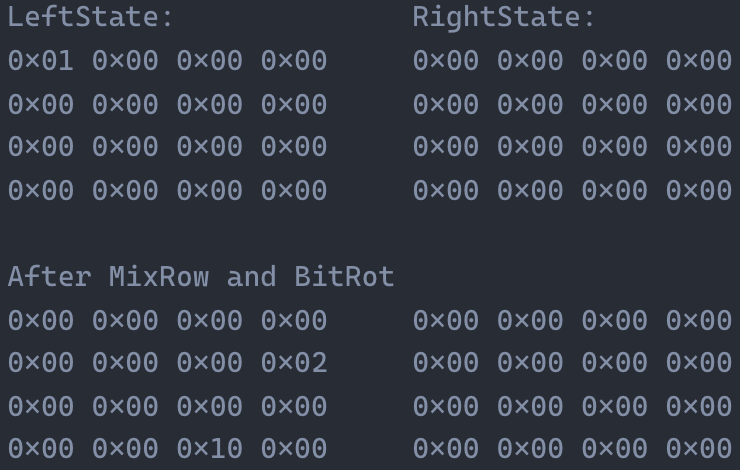
\includegraphics[width=1.0\textwidth]{Round1} %插入图片,[]中设置图片大小,{}中是图片文件名
    \caption{Round 1} %最终文档中希望显示的图片标题
    \label{Round1} %用于文内引用的标签
\end{figure}
After entering the Sbox, the $p_0$ state has the probibility of $2/8=2^{-2}$ to maintain 0x01. 

Maintain value probability $P_2=1/4=  2^{-2}$

\textbf{Round2}\\
\begin{figure}
    \centering %图片居中
    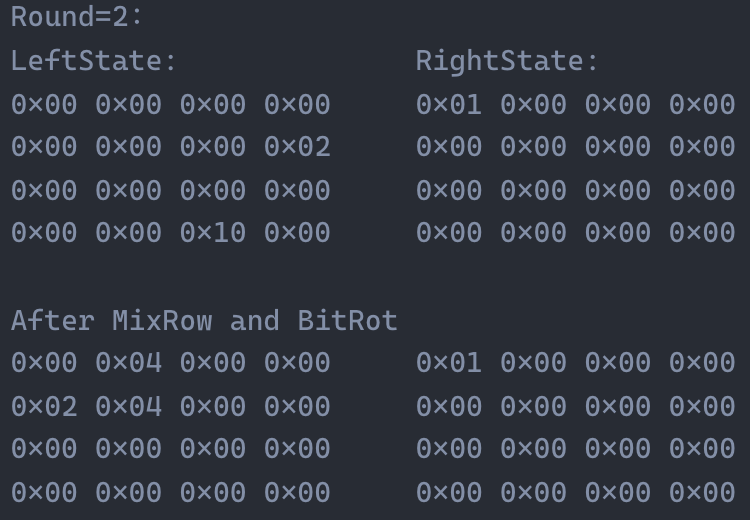
\includegraphics[width=1.0\textwidth]{Round2} %插入图片,[]中设置图片大小,{}中是图片文件名
    \caption{Round 2} %最终文档中希望显示的图片标题
    \label{Round2} %用于文内引用的标签
\end{figure}
We have 0x02 0x10 and 0x01.\\
Maintain value probability $P_2=1/4 * 1/4 * 1/4 = 2^{-6}$
 

\begin{table}[ht]
    \centering
    \setlength{\tabcolsep}{0.9mm}{
    \begin{tabular}{l|llllllllllllllllllllllllllllllll}
       & 0  & 1 & 2 & 3 & 4 & 5 & 6 & 7 & 8 & 9 & 10 & 11 & 12 & 13 & 14 & 15 & 16 & 17 & 18 & 19 & 20 & 21 & 22 & 23 & 24 & 25 & 26 & 27 & 28 & 29 & 30 & 31 \\ \hline
    0  & 32 & 0 & 0 & 0 & 0 & 0 & 0 & 0 & 0 & 0 & 0  & 0  & 0  & 0  & 0  & 0  & 0  & 0  & 0  & 0  & 0  & 0  & 0  & 0  & 0  & 0  & 0  & 0  & 0  & 0  & 0  & 0  \\
    1  & 0  & 8 & 0 & 8 & 0 & 8 & 0 & 8 & 0 & 0 & 0  & 0  & 0  & 0  & 0  & 0  & 0  & 0  & 0  & 0  & 0  & 0  & 0  & 0  & 0  & 0  & 0  & 0  & 0  & 0  & 0  & 0  \\
    2  & 0  & 0 & 8 & 0 & 0 & 0 & 8 & 0 & 0 & 0 & 8  & 0  & 0  & 0  & 8  & 0  & 0  & 0  & 0  & 0  & 0  & 0  & 0  & 0  & 0  & 0  & 0  & 0  & 0  & 0  & 0  & 0  \\
    3  & 0  & 4 & 0 & 4 & 0 & 4 & 0 & 4 & 0 & 4 & 0  & 4  & 0  & 4  & 0  & 4  & 0  & 0  & 0  & 0  & 0  & 0  & 0  & 0  & 0  & 0  & 0  & 0  & 0  & 0  & 0  & 0  \\
    4  & 0  & 0 & 0 & 0 & 8 & 0 & 0 & 0 & 0 & 0 & 0  & 0  & 8  & 0  & 0  & 0  & 0  & 0  & 0  & 0  & 8  & 0  & 0  & 0  & 0  & 0  & 0  & 0  & 8  & 0  & 0  & 0  \\
    5  & 0  & 4 & 0 & 4 & 0 & 0 & 0 & 0 & 0 & 0 & 0  & 0  & 0  & 4  & 0  & 4  & 0  & 4  & 0  & 4  & 0  & 0  & 0  & 0  & 0  & 0  & 0  & 0  & 0  & 4  & 0  & 4  \\
    6  & 0  & 0 & 4 & 0 & 0 & 0 & 4 & 0 & 0 & 0 & 4  & 0  & 0  & 0  & 4  & 0  & 0  & 0  & 4  & 0  & 0  & 0  & 4  & 0  & 0  & 0  & 4  & 0  & 0  & 0  & 4  & 0  \\
    7  & 0  & 2 & 0 & 2 & 0 & 2 & 0 & 2 & 0 & 2 & 0  & 2  & 0  & 2  & 0  & 2  & 0  & 2  & 0  & 2  & 0  & 2  & 0  & 2  & 0  & 2  & 0  & 2  & 0  & 2  & 0  & 2  \\
    8  & 0  & 0 & 0 & 0 & 0 & 0 & 0 & 0 & 8 & 8 & 0  & 0  & 0  & 0  & 0  & 0  & 0  & 0  & 0  & 0  & 0  & 0  & 0  & 0  & 8  & 8  & 0  & 0  & 0  & 0  & 0  & 0  \\
    9  & 0  & 0 & 0 & 0 & 0 & 0 & 0 & 0 & 4 & 0 & 0  & 4  & 4  & 0  & 0  & 4  & 0  & 0  & 0  & 0  & 0  & 0  & 0  & 0  & 4  & 0  & 0  & 4  & 4  & 0  & 0  & 4  \\
    10 & 0  & 0 & 4 & 4 & 0 & 0 & 4 & 4 & 0 & 0 & 0  & 0  & 0  & 0  & 0  & 0  & 0  & 0  & 0  & 0  & 0  & 0  & 0  & 0  & 0  & 0  & 4  & 4  & 0  & 0  & 4  & 4  \\
    11 & 0  & 4 & 4 & 0 & 0 & 4 & 4 & 0 & 0 & 0 & 0  & 0  & 0  & 0  & 0  & 0  & 0  & 0  & 0  & 0  & 0  & 0  & 0  & 0  & 0  & 4  & 4  & 0  & 0  & 4  & 4  & 0  \\
    12 & 0  & 0 & 0 & 0 & 4 & 4 & 0 & 0 & 0 & 0 & 0  & 0  & 4  & 4  & 0  & 0  & 0  & 0  & 0  & 0  & 4  & 4  & 0  & 0  & 0  & 0  & 0  & 0  & 4  & 4  & 0  & 0  \\
    13 & 0  & 0 & 0 & 0 & 4 & 0 & 0 & 4 & 4 & 0 & 0  & 4  & 0  & 0  & 0  & 0  & 0  & 0  & 0  & 0  & 4  & 0  & 0  & 4  & 4  & 0  & 0  & 4  & 0  & 0  & 0  & 0  \\
    14 & 0  & 0 & 2 & 2 & 0 & 0 & 2 & 2 & 0 & 0 & 2  & 2  & 0  & 0  & 2  & 2  & 0  & 0  & 2  & 2  & 0  & 0  & 2  & 2  & 0  & 0  & 2  & 2  & 0  & 0  & 2  & 2  \\
    15 & 0  & 2 & 2 & 0 & 0 & 2 & 2 & 0 & 0 & 2 & 2  & 0  & 0  & 2  & 2  & 0  & 0  & 2  & 2  & 0  & 0  & 2  & 2  & 0  & 0  & 2  & 2  & 0  & 0  & 2  & 2  & 0  \\
    16 & 0  & 0 & 0 & 0 & 0 & 0 & 0 & 0 & 0 & 0 & 0  & 0  & 0  & 0  & 0  & 0  & 8  & 8  & 8  & 8  & 0  & 0  & 0  & 0  & 0  & 0  & 0  & 0  & 0  & 0  & 0  & 0  \\
    17 & 0  & 0 & 0 & 0 & 0 & 0 & 0 & 0 & 0 & 0 & 0  & 0  & 0  & 0  & 0  & 0  & 4  & 4  & 4  & 4  & 4  & 4  & 4  & 4  & 0  & 0  & 0  & 0  & 0  & 0  & 0  & 0  \\
    18 & 0  & 0 & 0 & 0 & 0 & 0 & 0 & 0 & 0 & 0 & 0  & 0  & 0  & 0  & 0  & 0  & 4  & 4  & 0  & 0  & 0  & 0  & 4  & 4  & 4  & 4  & 0  & 0  & 0  & 0  & 4  & 4  \\
    19 & 0  & 0 & 0 & 0 & 0 & 0 & 0 & 0 & 0 & 0 & 0  & 0  & 0  & 0  & 0  & 0  & 2  & 2  & 2  & 2  & 2  & 2  & 2  & 2  & 2  & 2  & 2  & 2  & 2  & 2  & 2  & 2  \\
    20 & 0  & 0 & 0 & 0 & 4 & 0 & 4 & 0 & 0 & 0 & 0  & 0  & 4  & 0  & 4  & 0  & 0  & 0  & 0  & 0  & 0  & 4  & 0  & 4  & 0  & 0  & 0  & 0  & 0  & 4  & 0  & 4  \\
    21 & 0  & 4 & 0 & 4 & 0 & 0 & 0 & 0 & 0 & 0 & 0  & 0  & 0  & 4  & 0  & 4  & 4  & 0  & 4  & 0  & 0  & 0  & 0  & 0  & 0  & 0  & 0  & 0  & 4  & 0  & 4  & 0  \\
    22 & 0  & 0 & 4 & 0 & 4 & 0 & 0 & 0 & 0 & 0 & 4  & 0  & 4  & 0  & 0  & 0  & 0  & 0  & 0  & 4  & 0  & 4  & 0  & 0  & 0  & 0  & 0  & 4  & 0  & 4  & 0  & 0  \\
    23 & 0  & 2 & 0 & 2 & 0 & 2 & 0 & 2 & 0 & 2 & 0  & 2  & 0  & 2  & 0  & 2  & 2  & 0  & 2  & 0  & 2  & 0  & 2  & 0  & 2  & 0  & 2  & 0  & 2  & 0  & 2  & 0  \\
    24 & 0  & 0 & 0 & 0 & 0 & 0 & 0 & 0 & 4 & 4 & 4  & 4  & 0  & 0  & 0  & 0  & 0  & 0  & 0  & 0  & 0  & 0  & 0  & 0  & 4  & 4  & 4  & 4  & 0  & 0  & 0  & 0  \\
    25 & 0  & 0 & 0 & 0 & 0 & 0 & 0 & 0 & 2 & 2 & 2  & 2  & 2  & 2  & 2  & 2  & 0  & 0  & 0  & 0  & 0  & 0  & 0  & 0  & 2  & 2  & 2  & 2  & 2  & 2  & 2  & 2  \\
    26 & 0  & 0 & 0 & 0 & 0 & 0 & 0 & 0 & 4 & 4 & 0  & 0  & 0  & 0  & 4  & 4  & 4  & 4  & 0  & 0  & 0  & 0  & 4  & 4  & 0  & 0  & 0  & 0  & 0  & 0  & 0  & 0  \\
    27 & 0  & 0 & 0 & 0 & 0 & 0 & 0 & 0 & 2 & 2 & 2  & 2  & 2  & 2  & 2  & 2  & 2  & 2  & 2  & 2  & 2  & 2  & 2  & 2  & 0  & 0  & 0  & 0  & 0  & 0  & 0  & 0  \\
    28 & 0  & 0 & 0 & 0 & 2 & 2 & 2 & 2 & 0 & 0 & 0  & 0  & 2  & 2  & 2  & 2  & 0  & 0  & 0  & 0  & 2  & 2  & 2  & 2  & 0  & 0  & 0  & 0  & 2  & 2  & 2  & 2  \\
    29 & 0  & 0 & 0 & 0 & 2 & 2 & 2 & 2 & 2 & 2 & 2  & 2  & 0  & 0  & 0  & 0  & 0  & 0  & 0  & 0  & 2  & 2  & 2  & 2  & 2  & 2  & 2  & 2  & 0  & 0  & 0  & 0  \\
    30 & 0  & 0 & 2 & 2 & 2 & 2 & 0 & 0 & 0 & 0 & 2  & 2  & 2  & 2  & 0  & 0  & 0  & 0  & 2  & 2  & 2  & 2  & 0  & 0  & 0  & 0  & 2  & 2  & 2  & 2  & 0  & 0  \\
    31 & 0  & 2 & 2 & 0 & 2 & 0 & 0 & 2 & 2 & 0 & 0  & 2  & 0  & 2  & 2  & 0  & 2  & 0  & 0  & 2  & 0  & 2  & 2  & 0  & 0  & 2  & 2  & 0  & 2  & 0  & 0  & 2 
    \end{tabular}}
    \caption{Differential distribution table for 5-bit Sbox}
    \label{tab:Table2}
    
\end{table}

\end{homeworkProblem}
\end{document}


